
\documentclass[12pt]{article}
\usepackage[utf8]{inputenc}
\usepackage[T1]{fontenc}
\usepackage{amsmath, amssymb}
\usepackage{graphicx}
\usepackage{hyperref}
\usepackage{geometry}
\usepackage{listings}
\usepackage{xcolor}
\geometry{margin=1in}
\setlength{\parskip}{6pt}
\setlength{\parindent}{0pt}

\title{Numerical Demonstration of the Heisenberg Uncertainty Principle using Gaussian Wave Packets}
\author{Stefan Len \\ Independent Researcher \\ \texttt{tqe.simulation@gmail.com}}
\date{October 20, 2025}

\begin{document}

\maketitle

\begin{abstract}
I present a minimal numerical demonstration of the Heisenberg Uncertainty Principle using Gaussian wave packets in one spatial dimension. By systematically varying the initial position spread, I numerically verify the reciprocal relationship between position and momentum uncertainties and confirm that their product at the initial time achieves the theoretical minimum of $\hbar/2$. The results highlight the role of Gaussian wave packets as minimum-uncertainty states at the initial moment and provide an accessible, reproducible teaching tool for quantum mechanics.
\end{abstract}

\textbf{Keywords:} Heisenberg uncertainty principle, Gaussian wave packet, quantum mechanics, minimum uncertainty state, numerical simulation, pedagogical tool

\section{Introduction}
The Heisenberg Uncertainty Principle, formulated by Werner Heisenberg in 1927~\cite{heisenberg1927}, expresses a fundamental quantum constraint:
\[
\Delta x \cdot \Delta p \ge \frac{\hbar}{2}
\]
where $\Delta x$ and $\Delta p$ are position and momentum uncertainties. Gaussian wave packets achieve the minimum bound, making them ideal for illustrating the principle.

\section{Theory and Method}
A normalized Gaussian wave packet:
\[
\psi(x,0) = \left(\frac{1}{2\pi\sigma_x^2}\right)^{1/4} e^{-\frac{x^2}{4\sigma_x^2}}
\]
Its Fourier transform yields:
\[
\Psi(p,0) = \left(\frac{2\sigma_x^2}{\pi\hbar^2}\right)^{1/4} e^{-\frac{\sigma_x^2 p^2}{\hbar^2}}
\]
showing $\sigma_p = \hbar / (2\sigma_x)$ and $\Delta x \Delta p = \hbar/2$.

\section{Results}
\begin{figure}[h]
\centering
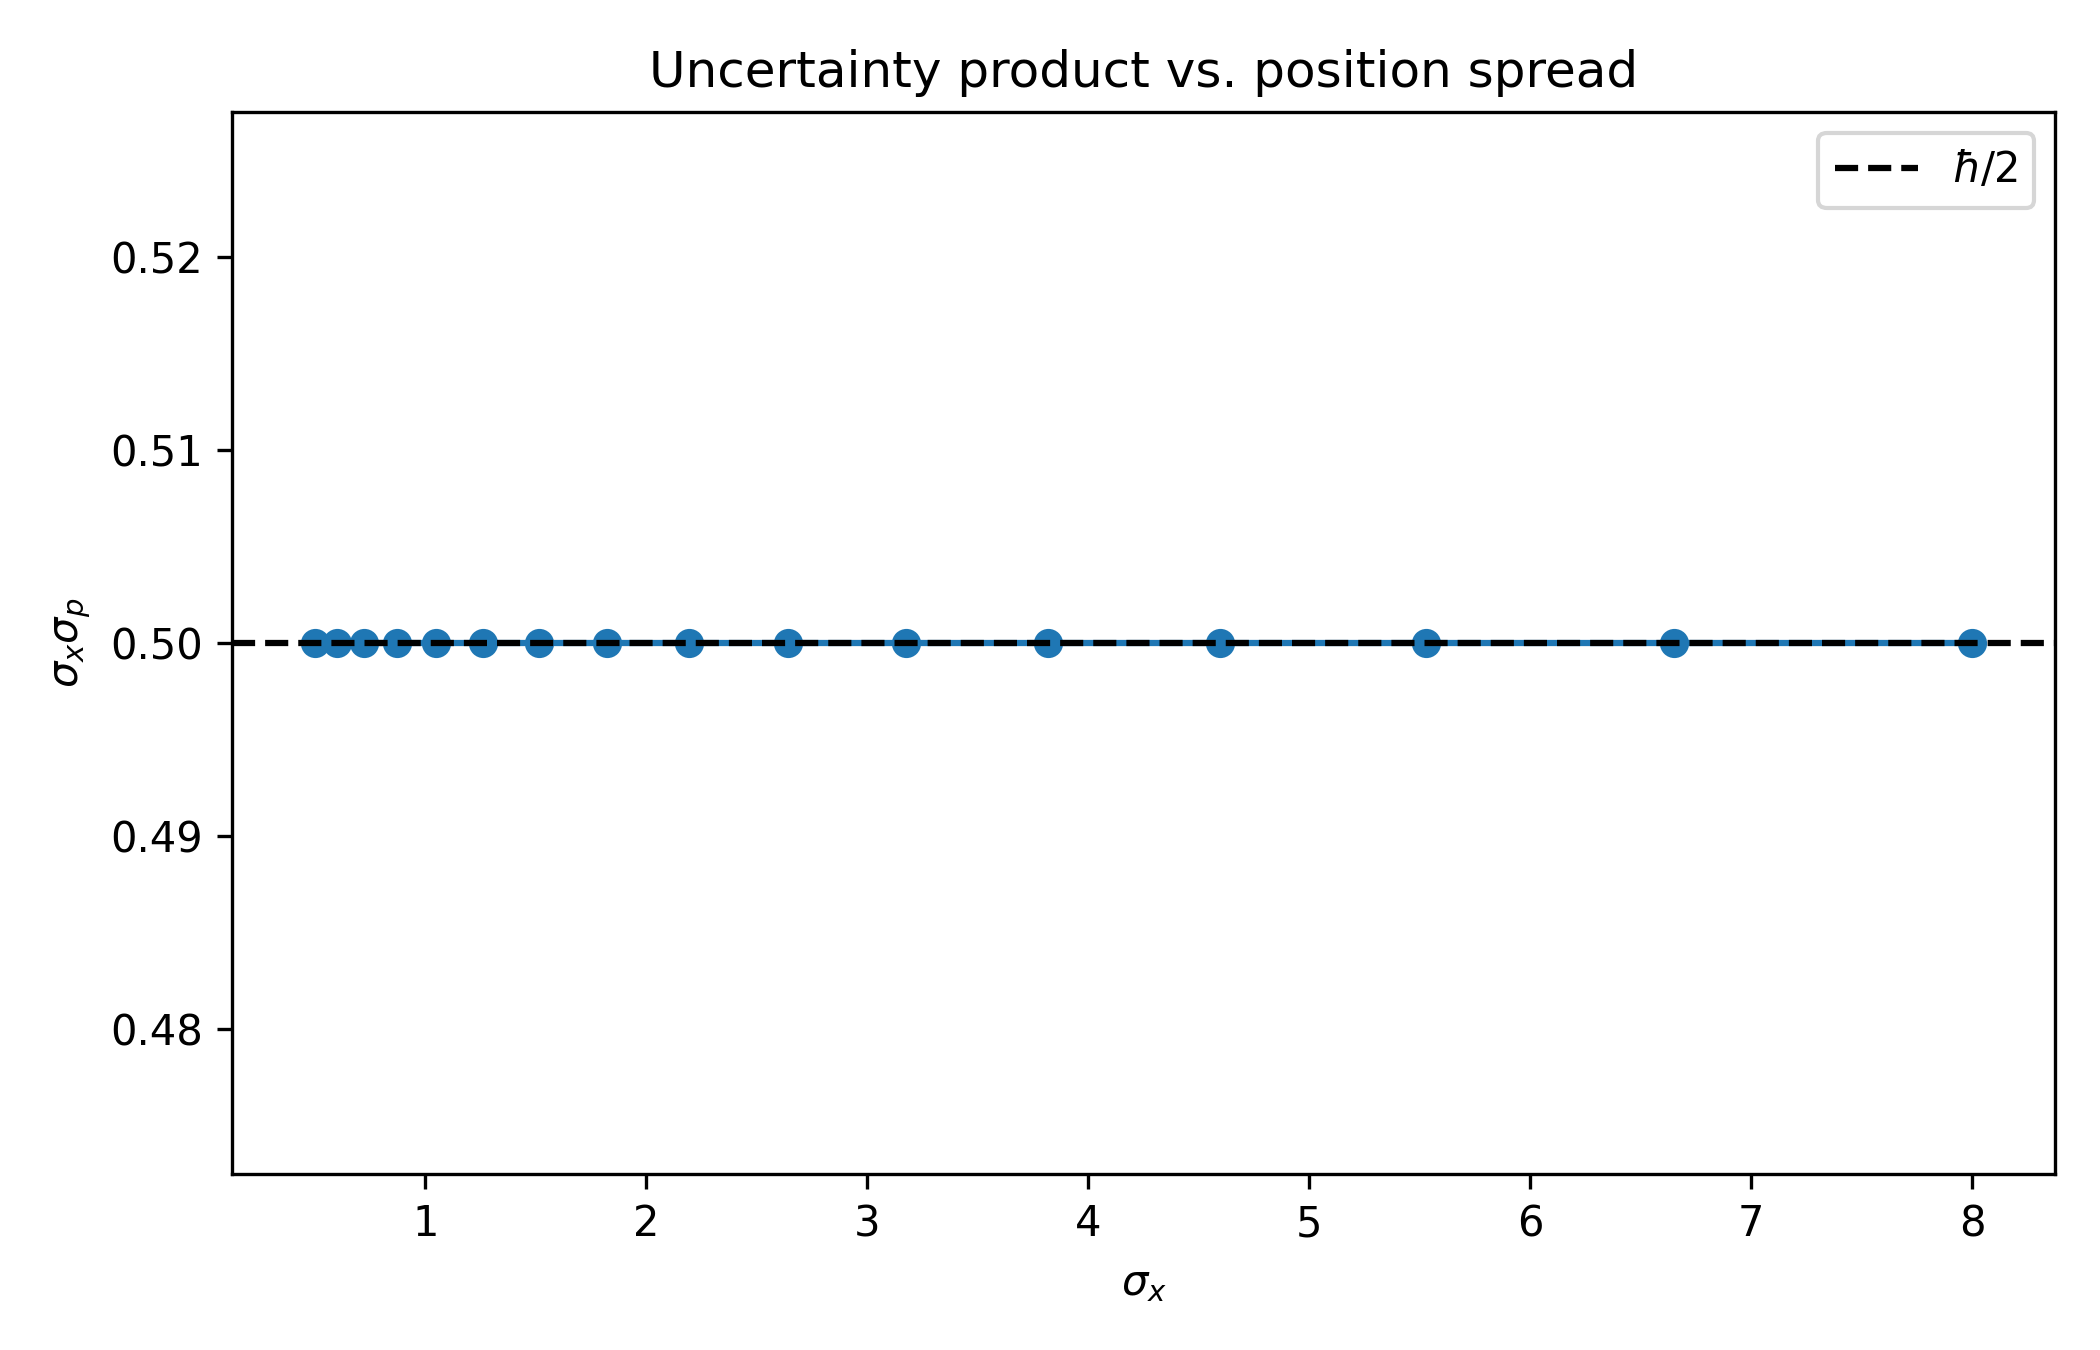
\includegraphics[width=0.8\linewidth]{figs/uncertainty_product.png}
\caption{Uncertainty product $\Delta x \cdot \Delta p$ as a function of $\sigma_x$. The constant $\approx 0.5$ confirms the Heisenberg limit.}
\end{figure}

The numerical results confirm $\Delta x \Delta p = \hbar / 2$ across all initial widths.

\section{Conclusions}
Gaussian wave packets numerically achieve the Heisenberg lower bound at $t=0$ and exhibit spreading over time while conserving momentum uncertainty. This provides a reproducible educational tool for quantum mechanics.

\section*{Acknowledgments}
Independent research by Stefan Len. Simulations implemented in Python (NumPy + Matplotlib).  
GitHub: \href{https://github.com/SteviLen420/Heisenberg_Uncertainty_Simulation}{repository link}.

\bibliographystyle{plain}
\begin{thebibliography}{9}
\bibitem{heisenberg1927} Heisenberg, W. (1927). \emph{Über den anschaulichen Inhalt der quantentheoretischen Kinematik und Mechanik}. Zeitschrift für Physik, 43(3-4), 172–198.
\bibitem{kennard1927} Kennard, E. H. (1927). \emph{Zur Quantenmechanik einfacher Bewegungstypen}. Zeitschrift für Physik, 44(4–5), 326–352.
\bibitem{robertson1929} Robertson, H. P. (1929). \emph{The Uncertainty Principle}. Physical Review, 34(1), 163.
\end{thebibliography}

\end{document}
